\chapter{Minimization of a Functional}
	
	A classical problem in minimization is the brachistrochrone, so the fastest ultimate curve (meaning determining the fastest trajectory to move from a point $A$ to a point $B$ considering that the only action is the one of the gravity).
	
	\textbf{MAGARI FARE LA FIGURA}
	
	Mathematically the problem is determining the curve $\mathcal C: [a,b] \rightarrow \mathds R$ such that $\mathcal C(a) = y_a$ and $\mathcal C(b) = y_b$ that minimize the function $T(\mathcal C)$ representing the time to travel and so
	\[ \textrm{minimize } T(\mathcal C) \qquad \textrm{for all possible curves } \mathcal C \]
	
	We can see that a \textbf{function} takes a number as input and returns a number, like $f(x) = x e^x$. A \de{functional} is instead something that takes as input a function and returns a number and an example is
	\[ \mathcal F (x) = \int_a^b x(t)\, dt  \]
	where $x$ is a function. Considering for example $x(t) = t^2$ the previous functional  becomes
	\[ \fun F(x) = \int_a^b t^2\, dt = \left. \frac{t^3}{3}\right|_a^b= \frac{b^3-a^3}{3}\]
	
	Another example of functional can be $\fun G(z) = z'(0) \int_0^1 z^2(t)\, dt$ and this expression can be evaluated for every generic function $z(t)$.	\vspace{3mm}
	
	The question of this problem is how to define a \textit{minimum} for a functional; in order to do so we have to firstly understand how to minimize a simple function and in particular given a function $f: A\subseteq \R \rightarrow \R$ has a minimum in the point $x^*$ if
	\[  f(x^*) \leq f(x) \qquad \forall x \in A \]
	Similarly given a function $\fun F(x)$ a \textit{point} $x^*$ (that in reality is a function) is a minimum if 
	\[ \fun F(x^*) \leq \fun F(x) \qquad \forall x \in ? \]
	In this case we have to specify the \textit{class} (functional space) of functions we are considering, as example $x$ can be a function that's continuous in the domain $[a,b]$ and so we can define
	\[ x\in C([a,b]) = \big\{ g:[a,b]\rightarrow R \ | \ g \textrm{ is continuous} \big\} \]
	In general changing the \textit{domain} of the functional $\fun F$ may change the problem.
	\begin{example}{: domain change}
		Considering the function $f(x) = x^2+2$, it's roots can be computed if we allow complex solutions $z\in \mathds C$ (and in fact $z = \pm i \sqrt 2$), while if the domain of the solution is the real set $z\in \R$ no solutions exists. \vspace{3mm}
		
		Considering now the functional $\fun F$ defined as
		\[ \fun F(x) = \int_{-1}^1 \big(x(t) - |t|\big)^2\, dt \]
		The $|t|$ introduce a cuspid in $t=0$ that cannot be derived. If we minimize the functional in the continuous interval $x\in C([-1,1])$, the solution is the function $x^*(t) = |t|$, in fact
		\[ \fun F(x^*) = \int_{-1}^1 \big(|t|-|t|\big)^2 \, dt = \int_{-1}^1 0\, dt = 0 \]
		Choosing any other continuous function will result in a functional with a positive value.
		
		Considering now to minimize the function in the domain of functions with continuous derivatives, and so $x\in C^1([-1,1])$. In this case $|t|\notin C^1([-1,1])$ (due to the cuspid). An approximation of the function $|t|$ that is continuous with also continuous first derivative is the function
		\[ x_\varepsilon(t) = \begin{cases}
			t \qquad & t \geq \varepsilon \\
			\frac 1 2 \left(\frac{t^2}\varepsilon + \varepsilon\right) \qquad & -\varepsilon < t< \varepsilon \\
			-t & t \leq- \varepsilon
		\end{cases} \]
		By pushing the limit $\varepsilon\rightarrow 0$ we can have the function that minimize the functional $\fun F$ in the domain $C^1([-1,1])$. In fact we can see that the functional of $x_\varepsilon$ becomes
		\[ \fun F(x_\varepsilon) = \int_{-\varepsilon}^\varepsilon \left( \frac{t^2}{2\varepsilon} + \frac \varepsilon 2 - |t| \right)^2\, dt = \frac{\varepsilon^3}{10} \]
		
	\end{example}

	\paragraph{Relations with linear algebra} To analyse the functionals we use the concept of scalar product (from linear algebra) and norm extended to the vector spaces of functions. As example considering the set $\mathcal V = \big\{ f: [0,1]\rightarrow \R \textrm{ continuous} \big\}$, then $\mathcal V$ is a vector spaces where the \textit{vectors} are the continuous function and the \textit{scalars} are the real number. With this said fiven the vectors $f(x) = x^2$ and $g(x) = \sin x$, than using the linear property another vector can be created as
	\[ f(x) + g(x) = x^2 + \sin x \]
	A vector space is \textit{closed} for the operation of vector summations and multiplication by a scalar, and in fact any combination $\alpha f(x) + \beta g(x)$ ($\forall \alpha,\beta\in \R$) is inside the vector space $\mathcal V$. An example of a scalar product in $\fun V$ is the following relation
	\[ \langle f,g\rangle = \int_0^1 f(x)g(x)\, dx \]
	We can prove this identity considering the bi-linear property in the vectorial space:
	\textbf{RISCRIVERE QUESTA DEFINIZIONE}
	
	We can also compute the norm of the function $f$ as
	\[ \|f\| = \sqrt{\langle f,f\rangle} = \sqrt{\int_0^1 f^2(x)\, dx} \]
	Clearly $\|f\| \geq 0$ and $\|f\| = 0$ if and only if $f(x) = 0$. 
	
	\begin{example}{: space of function}
		A space of functions can ve the one $f:[a,b]\rightarrow \R$ such that $f$ is continuous, or for example $f:[a,b]\rightarrow \R$ where $f\in C^k([a,b])$ (for $k\in \mathds N$). The same can be said for piecewise continuous functions.
		
		Less trivially is a space of function the set of $f:[a,b]\rightarrow \R$ that are module integrable, and so all the function $f$ such that
		\[\int_a^b |f(x)|\, dx < \infty\]
		
	\end{example}

	In general we define as $L^p([a,b])$ the space of $p$-integrable functions, so such that
	\[ f\in L^p([a,b])  \qquad \Leftrightarrow \qquad \int_a^b |f(x)|^p\, dx < \infty\]
	
	
	\paragraph{Directional derivative} The minimum of a bidimensional function $f(x,y)$ is the point $(x^*,y^*)$ that satisfy $f(x^*,y^*)\leq f(x,y)$ for all $(x,y)\in \R^2$.
	
	We can now introduce the function $g(t) := f(x^* + t\, dx, y^* + t\, dy)$ where $\vett d = (dx,dy)$ is an arbitrary direction, than we have that
	\[ g(0) = f(x^*,y^*)\leq f(x,y) \qquad \Rightarrow \quad \frac{g(t)-g(0)}{t} \geq 0 \qquad \forall t\geq 0\]
	By pushing the limit we can see that
	\[ \lim_{t\rightarrow 0}\frac{g(t)-g(0)}{t} = g'(0) \geq 0 \]
	
	\textbf{RISCRIVERE ESPANSIONE DI TAYLOR}
	
	\paragraph{Minimum for a functional} To define a stationary point of a functional $\fun F: f(\cdot)\rightarrow \R$, let $x^*(t)$ a function that \textit{minimize} the $\fun F$ and $y(t)$ another function so such that
	\[ \mathcal F(x^*) \leq \mathcal F(y) \]
	We can try to \textit{connect} the two points determined by the function $x^*$ and $y$ using a straight line, determining the function
	\[ z(t,\tau) = x^*(t) + \tau\underbrace{\big(y(t)-x^*(t)\big)}_{\textrm{direction}} \]
	We can see that for $\tau = 0$ then $z(t,0)=x^*$ while $z(t,1) = y(t)$. Defining the direction $d(t) = y(t)-x^*(t)$ then the previous relation can be rewritten as
	\[ z(t,\tau) = x^*(t) + \tau \, d(t) \]
	Defining now the \textit{slice} of the function along the function $z$, we can compute the function
	\[ g(\tau) = \fun F\big(z(\cdot,\tau)\big) = \fun F\big(x^* + \tau \, d\cdot\big) \]
	In this case $g:\R\rightarrow \R$ can be easily analysed and with the original assumptions done than $g(0) = \mathcal F(x^+) \leq g(\tau) = \fun F(x^++ \tau \, d\cdot)$. Then if $g'(0)$ exists, it means that
	\begin{align*}
		g'(0) & \lim_{t\rightarrow 0} \frac{g(t)-g(0)}{t} \geq 0
	\end{align*}

	If we also consider that $f(x,y)$ is a function that has a Taylor series as
	\[ f\big(x\s + t\, dx,y\s+t\, dy\big) = f\big(x\s,y\s\big) + \nabla f\big(x\s,y\s\big) \vector{t\, dx \\ t \, dy} + \mathcal O(t^2) \]
	and that we can relate
	\begin{align*}
		\frac{g(t)-g(0)}{t} & = \frac{f\big(x\s + t\, dx,y\s+t\, dy\big) - f\big(x\s,y\s\big)}{t} \\& = \nabla f\big(x\s,y\s\big) \vector{dx \\ dy} + \mathcal O(t^2) \geq 0
	\end{align*}
	If we now choose as direction to compute the derivative the opposite one of the gradient, and so $\vett d = - \nabla f(x\s,y\s)^t$ we have that
	\[ \nabla f(x\s,y\s) \Big(-\nabla f(x\s,y\s)\Big)^t = - \|\nabla f(x\s,y\s)\|^2 \geq 0 \]
	and so this implies that the derivative $\nabla f(x\s,y\s)$ is necessarily zero.
	000
	The conclusion of the process it that if $x^*$ is a \textit{minimum point}, then every directional derivative of $x^*$ is equals to 0. While performing this operation we have to consider that each  generated function $x\s+\tau\, d\cdot$ must be \textit{feasible}.
	
	
	\begin{example}{}
		Given the functional
		\[ \fun F(x) = \int_0^1 x^2(t) + 1 \, dt  \ + x(1) \]
		if we try to compute the generic directional derivative of a function $x(t)$ with direction $d(t)$, then $z(t,\alpha) = x(t) + \alpha d(t)$ and so 
		
		\textbf{RISCRIVERE L'ESEMPIO} 
	\end{example}
	
\section{Fundamental lemma of the calculus of variations}
	{\itshape Given a function $f:[a,b]\rightarrow \R$ (piecewise continuous) such that for all $g:[a,b] \rightarrow \R, g \in C^\infty([a,b])$ with $g(a) = g(b) = 0$ and $g^{(k)}(a) = g^{(k)}(b) = 0 \ \forall k$, if the integral 
	\begin{equation} \label{eq:func:lemma}
		\int_a^b f(x)\,g(x) \, dx = 0
	\end{equation}
	then $f(x)= 0 $ is identically null. }

	\paragraph{Lemma: sign permanence} In order to later proof the fundamental lemma yet described, we have to remark the \textit{sign permanence} that states: {\itshape given a function $f:[a,b]\rightarrow \R$ continuous such that $f(c) >0$, then there exists a $\delta >0$ such that }
	\[ f(x) \geq \frac{f(c)}{2} \qquad \forall x \in [c-\delta,c+\delta] \]
	
	The proof of this lemma can be done defining the parameter $\epsilon = f(c) / 2$; based on the assumption that $f(x)$ is continuous, then $\exists\, \delta >0$ such that 
	\[ |f(x) - f(c)| \leq \varepsilon \qquad \forall |c-x|\leq \delta \]
	
	\textbf{FINIRE LA DIMOSTRAZIONE}
	
	\paragraph{Proof of the fundamental lemma} The proof of the fundamental lemma of the calculus of variation can be done by contradiction. Let consider the integral $\int_a^b f(x) g(x)\, dx = 0$ for all functions $g(x)$ and such that, given the function $f$, exists a point $c$ such that $f(c) > 0$ (in general the proof can be done for $f(c)\neq 0$). from the sign permanence lemma we can state that exists an interval $[c-\delta,c+\delta]$ such that $f(x) \geq \frac{f(c)}{2 } \geq 0$. Determining the function $g$ as
	\[ g(x) = \begin{cases}
		\dfrac{x-(c-\delta)}{\delta} \qquad & x\in [c-\delta, c] \\
		\dfrac{c-x+\delta}{\delta} & x\in[c,c+\delta] \\
		0 & \textrm{otherwise}
	\end{cases} \]
	Note that this function is continuous but $g\notin C^\infty$ (later will be described a function that presents this feature). With this definition the integral $\int_a^b fg\, dx$ so becomes
	\begin{align*}
		\int_{c-\delta}^{c+\delta} f(x)g(x)\, dx & \geq \frac{f(c)}{2} \int_{c-\delta}^{c+\delta} g(x)\, dx \\
		& \geq \frac{f(c)}{2}\frac \delta 2 > 0
	\end{align*}
	We can clearly see that the integral $\int_a^b fg\, dx$ has a positive real value grater than zero that's (considering that $f$ has at least on point $c$ such that $f(c) >0$) in contraposition with the initial request that the integral should have been zero evaluated. \vspace{3mm}
	
	To create a direction function $g$ that's in the set $C^\infty$ we can use the function $h$(for whose those condition is demonstrated) as in figure \ref{fig:func:ht} defined as:
	\begin{equation} \label{eq:func:ht}
		h(t) = \begin{cases}
			e^{-1/t} \qquad & t > 0 \\ 
			0 & t\leq 0
		\end{cases}
	\end{equation}
	\begin{SCfigure}[2][bt]
		\centering 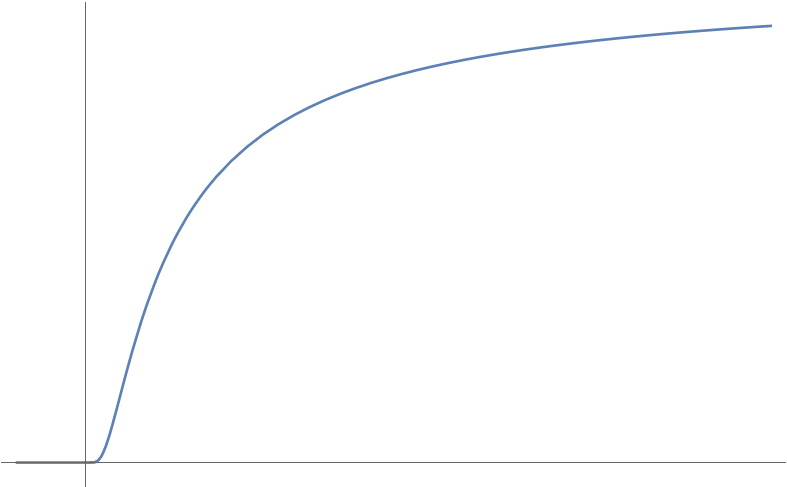
\includegraphics[width=4cm]{cinf-a}
		\caption{representation of $h(t)$ defined in equation \ref{eq:func:ht}}.
		\label{fig:func:ht}
	\end{SCfigure}

	A way to create a function that presents a \textit{bell shape} in the range $[0,1]$ is by computing $g(t) := h(t) h(1-t)$ how's graph in the range $[0,1]$ is similar to the one shown in figure \ref{fig:func:hbell}.
	
	\begin{SCfigure}[2][bht]
		\centering 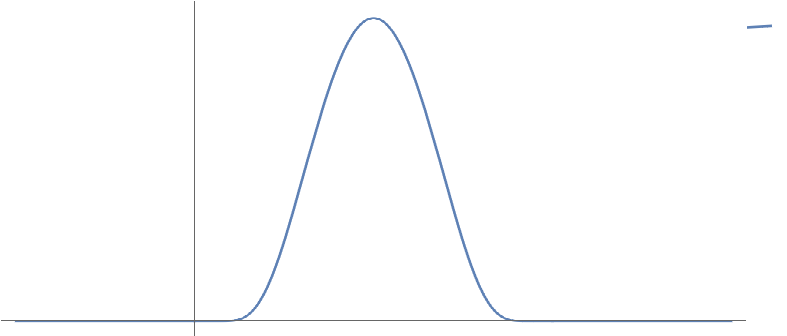
\includegraphics[width=4cm]{cinf-b}
		\caption{representation of the function $g(t):=h(t)h(1-t)$, where $h(t)$ is defined in equation \ref{eq:func:ht}}.
		\label{fig:func:hbell}
	\end{SCfigure}
	
	In particular to demonstrate the fundamental lemma of the calculus of variations we need to rescale the function $g$ in order to have a bell centered in the point $c$ with a \textit{bell width} $\delta$ and so we consider
	\[ g(t) = K \, h\left(\frac{t-c+\delta}{2 \delta}\right) h\left( \frac{\delta + c - t}{2 \delta} \right) \] 
	where the constant $K\in\R$ is such that $g(c)=1$ and $\int_a^bg(x)\, dx$. In this case we can see that $g\in C^\infty$, $g(x) \geq 0 $ for all value $x$ and specifically $g(x) = 0 \, \forall x\notin[c-\delta,c+\delta]$.\\
	The lemma can now be proven by contradiction; as in the previous case if we consider a function $f$ that's not identically null (and in this case we assume that there is at least one point $c$ on which $f$ is positive), then we can state that (for the sign permanence theorem)
	\[ f(x) \geq \frac{f(c)}{2} \qquad \forall x \in [c-\delta,c+\delta] \] 
	We can now see that the original integral $\int_a^b fg\, dx$ is not equal to zero, in fact
	\[ \int_a^b f(x)g(x)\, dx \geq \frac{f(c)}{2}\int_a^bg(x)\, dx > 0 \]
	because $g(x)$ is always greater or equal to zero, determining a non zero value as result as in the previous case.
	
\section{Euler Lagrange equation}
	\paragraph{Pendulum example} The \de{Euler Lagrange equation} is the generalization of the minimum action principle that's used in physics. Considering as a practical example the motion of a pendulum of a mass $m$ that's free to oscillate in respect to a pivot point using a rope of length $l$, the kinetic energy $T$ and the potential term $V$ of the system can be expressed as
	\[ T = \frac 1 2 m v^2 \qquad \qquad \qquad V = mgy \]
	Considering $\theta$ as the angle that the rope determines with the vertical axis, then the we can rewrite the energies as functions of the angular position $\theta$ and velocity $\dot \theta$ as
	\[ T(\theta,\dot \theta) = \frac 1 2 m l^2 \dot\theta^2 \qquad \qquad \qquad V(\theta) = - m gl\sin\theta \]
	
	To solve the dynamic equation $\theta(t)$ of the mechanism we can compute the lagrangian $\mathcal L$ of the system defined as
	\[ \mathcal L(\theta,\dot\theta) = T(\theta,\dot\theta)-V(\theta) = \frac m 2 l^2\dot\theta^2 + lmg\cos\theta \]
	As law that's analyzed in mechanics physics we can state that the solution of the dynamics of the system is the one the function that minimize the \textbf{action} $\mathcal A$ of the system defined as
	\begin{equation} \label{eq:func:action}
		A(\theta) = \int_{t_0}^{t_1} \mathcal L(\theta,\dot\theta)\, dt
	\end{equation}
	where the values $\theta(t_0)= \theta_0$ and $\theta(t_1)=\theta_1$ are known parameters.
	
	In practice to determine the required solution we can use analytical tool to find the trajectory that can then be demonstrated to be the minimum of the action $\mathcal A$ (that's indeed a functional).
	
	However we can also try to analytically determine the function $\theta^*(t)$ that minimize the functional $\fun A(\cdot)$ by computing the directional derivatives. \vspace{3mm}
	
	Let now consider the function $\theta\s(t)$ and a direction $\delta_\theta$ that satisfy $\delta_\theta(t_0)=\delta_\theta(t_1) = 0$, we can then use the fundamental lemma of the calculus of variation to determine the minimal function (considering that the expression \ref{eq:func:action} of the action is comparable to equation \ref{eq:func:lemma} of the lemma).\\
	To determine the minimum point we have in fact to determine the function whose derivative is zero for each direction of approach to the point, and so in this example we need to compute
	\begin{align*}
		\frac{d}{d\alpha} \mathcal A\big(\theta\s + \alpha\, \delta_\theta\big) & = \frac{d}{d\alpha}\int_{t_0}^{t_1} \mathcal L \big( \theta \s + \alpha\, \delta_\theta, \dot\theta\s + \alpha\, \dot \delta_\theta \big) \\
		& = \int_{t_0}^{t_1} \left[\pd{}{\theta} \mathcal L( \dots ) \frac{d}{d\alpha}\big(\theta\s + \alpha \,\delta_\theta\big) +\pd{}{\dot\theta} \mathcal L (\dots) \frac{d}{d\alpha}\big(\theta\s + \alpha \,\dot \delta_\theta\big) \right]\, dt \\
		& = \int_{t_1}^{t_2} \left[ \big(-lmg\sin(\theta\s + \alpha\, \delta_\theta)\big)\delta_\theta + ml^2\big(
		\dot\theta\s + \alpha \, \dot\delta_\theta^2 \big)\, \dot\delta_\theta \right] \, dt
	\end{align*}
	Note that from in the first step we made the implicit assumption that $ \frac d{d\cdot} \int = \int\frac{d}{d\cdot}$ while however this is not always possible. Evaluating the previous expression for $\alpha = 0$ we can state that
	\[ 	\frac{d}{d\alpha} \mathcal A\big(\theta\s + \alpha\, \delta_\theta\big) \Big|_{\alpha = 0} = \int_{t_0}^{t_1} \big(-lmg \sin\theta\s\delta_\theta + ml^2\dot\theta\s \dot\delta_\theta \big) \, dt = 0 \qquad \forall \delta_\theta \]
	Performing an integration by part allows to remove the term $\dot\delta_\theta$ that's hard to determine, and in fact
	\[ \frac{d}{dt}\big( ml^2\dot\theta\s \, \delta_\theta\big) = \frac{d}{dt}\big(ml^2\dot\theta\s\big)\,\delta_\theta + ml^2\theta^{*2} \dot\delta_\theta\]
	\begin{align*}
		\Rightarrow \quad \left. \frac{d\mathcal A}{d\alpha}\right|_{\alpha = 0} & = \int_{t_0}^{t_1} \text{\textbf{RISCRIVERE}} \\
		& = \int_{t_0}^{t_1} \underbrace{\left[ -lmg \sin\theta\s - \frac d{dt}\big(ml \dot\theta^{*2}\big) \right]}_{f(t)} \delta_\theta\, dt = 0
	\end{align*}
	We can now see in this formulation that the marked expression represent the function $f$ of the fundamental lemma considering that the relation must be true for all approaching direction $\delta_\theta$, and so it must be
	\[ -lmg \sin\theta\s - \frac d{dt}\big(ml \dot\theta^{*2}\big) = 0 \]
	The problem now to complete the analyses of the pendulum motion is determining the function $\theta\s(t)$ that satisfy this expression and also match the boundary conditions $\theta(t_0) = \theta_0$ and $\theta(t_1)=\theta_1$.000
	
\subsection{General formulation}
	
	
	
	
	
	
	
	
	
	